\documentclass[oneside, final, 12pt]{extreport}
\usepackage{amsmath, amsthm, amssymb} %math expressions, theoreme/lemma, math symbols
\usepackage{mathtext} %russian letters in formulas

% fonts and lang
%\usepackage[T1,TS1,T2A]{fontenc}
\usepackage{cmap}
\usepackage[T1, T2A]{fontenc}
\usepackage[utf8]{inputenc}
\usepackage[english, russian]{babel}
%\usepackage{pscyr}    шрифты, мб не нужны, но они в любом случае пока не работают


% formatting
\usepackage{geometry} %customize page layout
\geometry{left = 3cm}
\geometry{right = 1cm}
\geometry{top = 1.5cm}
\geometry{bottom = 2cm}

\usepackage{setspace} %set space between lines
\usepackage{indentfirst} %indent first paragraph after section header
\usepackage{fancyhdr} %headers and footer
\usepackage{nopageno} %hiding page numbers where needed
\usepackage{tocloft} %control table of contents, figures

\usepackage{graphicx}

\linespread{1.3} %1.5 spacing


%Разработка метода прогнозирования слабой масштабируемости суперкомпьютерных приложений


%разобраться с правильным оформлением ссылок	
\begin{document}

	%титульный лист

	%\tableofcontents
	%\clearpage

	%\chapter{Введение}
	Без параллельных технологий сейчас невозможно обойтись во многих прикладных областях науки: гидро- и аэро- динамике, квантовая химии, сейсмике, компьютерном моделировании лекарств, криптографии и многих других. Это связано с необходимостью обрабатывать большие объёмы данных и производить колоссальное количество вычислений. Что стимулирует создание больших суперкомпьютерных центров, развитие технологий конструирования аппаратных комплектующих, разработку новых методик и алгоритмов.

	Если используемые пакеты прикладных программ и научные приложения будут плохо написаны, выбранный алгоритм слабо параллелизуем или неоптимально реализован в коде, то они не смогут в полной мере использовать вычислительные ресурсы, продоставляемые высокопроизводительным центром. Если рассмотреть результеты запусков бенчмарков HPL и HPCG на суперкомпьютерах из рейтенга TOP500 \cite{top500}, то окажется, что для HPL среднее отношение реальной и пиковой производительностей около 63.5\%, для HPCG этот показатель сильно ниже - около 1.5\%(результаты тестирования HPCG предоставлены только для 70 суперкомпьютеров).\#АКТУАЛЬНО но 16 марта\# Данные бенчмарки - это сверх оптимизированные приложения, написанные в тесном сотрудничестве математиками и программистами, лишь малая часть параллельных программ имеют схожую степень параллелизуемости.

	!!!ДАННЫЕ ОБ эффективности ИСПОЛЬЗОВАНИя пользователями ЛОМОНОСОВА1-2 или любого друго СК цента.!!!

	% фундаментальные ограничения, как закон Амдала и закон Густавсона — Барсиса,

	%Поэтому так важно иметь метрику, способную описать, как конфигурация системы и размер задачи влияют на производительность суперкомпьютеров и параллельных алгоритмов.

	Существует множество характерискик работы параллельных программ, например, время её выполнения, ускорение и эффективность, производительность, количество обращений в память и кэш-промахов. Все они имеют динамическую сущность, то есть могут изменяться от запуска к запуску, зависят от параметров запуска программы и машины, на которой она выполняется, поэтому будем называть их динамическими характеристиками параллельной программы.

	Чтобы понять свойства параллельных программ и причины найденных в них особенностей, нужно рассматривать все доступные динамические характеристики на всём пространстве параметров запуска. Этот задача напрямую связана с понятием "<масштабируемость">, свойством параллельной программы, характеризующим зависимость изменения всей совокупности динамических характеристик работы этой программы от множества параметров её запуска \cite{scalability_def}.

	Здесь и далее обозначим: \(p\) - количество процессов, на которых запущено приложение; \(N\) - размера задачи; \(T_A(N)\) - сложность алгоритма \(А\) для значения \(N\) размера входа. \(T_A(N) = \max_{||y|| = N} C^T_A(y)\), где \(C^T_A(y)\) сложность алгоритма \(А\) для входа \(y\) \cite{COMPLEXITY}. Сложность алгоритма следует понимать, как последовательную сложность, то есть, как число операций, которое нужно выполнить при последовательном выполнении алгоритма.

	Во время исследования масштабируемости приложения необходимо указывать, на какой области изменения значений параметров проведены запуски. По выбору параметров запуска, которые будут изменяться, масштабируемость согласно \cite{scaling_types} можно разделить на три основных типа:
	\begin{itemize}
		\item Сильная масштабируемость (strong scaling) - зависимость динамических характеристик от количества процессов \(p\) при фиксированной вычислительной сложности задачи задачи \((T_A(N) = const \Rightarrow N = const)\).
		\item Слабая масштабируемость (weak scaling) - зависимость динамических характеристик от количества процессов \(p\) при фиксированной вычислительной сложности задачи в пересчете на один узел \((T_A(N)\:/\:p = const)\)
		\item Масштабируемость вширь (wide scaling) - зависимость динамических характеристик от размера задачи при фиксированном количестве процессов \((p = const)\)
	\end{itemize}

	Масштабируемость - ключевое понятние в вопросах исследования свойств параллельных программ, поэтому крайне важно учитывать её на всех этапах разработки программного обеспечения. Однако не всегда возможно получить в распряжение большое количество узлов, чтобы увидеть характер изменения различных динамических характеристик приложения с ростом числа используемых узлов, при увеличении размера задачи, или ожидание этого может занять непозволительно много времени, например, авторы статьи \cite{log_main} утверждают, что в худшем случае время ожидания выделения необходимого количества узлов растёт экспоненциально с ростом количества запрашиваемых ресурсов системы. Но ведь именно возможность решать задачи больших размеров за разумное время, используя большое количество узлов, является главным преимуществом суперкомпьютерных систем, поэтому необходимо, чтобы приложение было хорошо масштабируемо. Обычно пользователь может выполнить задачу на небольшой конфигурацие быстрее, чем запустить на большом количестве узлов. Исходя из этого, актуальна задача прогнозирования масштабируемости приложения на большие конфигурации вычислительной системы, без доступа к его коду и возможности его изменять, основываясь только на данных, полученных из множественных запусков на малых конфигурациях. В данной работе предлагается механизм решения поставленной задачи в условиях слабой масштабируемости суперкомьютерных приложений.

%\clearpage
	\chapter{Постановка задачи}
	В данной работе поставлены следующие задачи:
	\begin{itemize}
		\item Разработать метод предсказания слабой масштабируемости суперкомпьютерных приложений.
		\item Провести эксперименты(ИЛИ собрать экспериментальную базу) и проверить применимость метода, оценить(ИЛИ оценив) точность предсказаний.
		\item Разработать программное средство позволяющее строить прогноз в соответствии с разработанным методом.(НЕ ОЧЕНЬ НРАВИТСЯ ФОРМУЛИРОВКА)
	\end{itemize}


\clearpage
	\chapter{Обзор существующие методов и подходов к предсказанию масштабируемости}
%как свойства параллельной программы, характеризующего зависимость изменения всей совокупности динамических характеристик работы этой программы от множества параметров её запуска
	Когда говорят о предсказании масштабируемости\#REF\#, то рассматривают не всю "<совокупность динамических характерискик работы"> программы, а её часть. Большинство исследований направлены на предсказание времени исполнения программы в зависимости от параметров её запуска, но также существуют другие, направленные на предсказание производительности, ускорения и эффективности, энергопотребления. Однако этими характеристиками всё не ограничивается, так, например, в работе \cite{efficiency_prediction} авторы строят модель, предсказывающую несколько не совсем стандартных характеристик параллельной программы: первая отражает потенциальную потерю эффективности, вызванную различными временами вычислений разных процессов, вторая - неэффективность, вызванную зависимостями в коде, а третья - потерю производительности, вызванную передачей данных.
	%Ими также как и в \#LINK\# исследуется возможность предсказания данных характеристик приложения на больших конфигурациях, построенного на основе запусков на малых конфигурациях. \#мб результаты убрать\# Модель тестируется с помощью приложений из CORAL(HACC, Nekbone, AMG2013) и приложения AVBP. Запуски HACC и Nekbone проводятся в условиях сильной масштабируемости, а AMG2013 и AVBP - в условиях слабой. Получившиеся значения относительных ошибок варьируются от 0.01\% до 27.19\%.

	Существует большое число работ направленых на исследование и предсказание масштабируемости приложений на суперкомпьютерах, но встречаются и такие, которые используют для запуска параллельных приложений отдельные узлые, небольшие вычислетельные системы, грид-системы, платформы для облачных вычислений.

	Все исследования можно разделить на две группы, первая объединяется в себе те, что ставят перед собой цель используя запуски на малых конфигурациях экстраполировать их на большие, вторая же состоит из тех работ, что основываясь на результатах запусков, равномерно распределённых по пространству параметров, пытаются интерполировать их на всё пространство параметров.

	Наиболее распространёнными для предсказания масшатибуемости являются подходы, использующие аппарат линейной регрессии, методы машинного обучения и нейронные сети, а также симуляцию исполнения программы или коллаборативную фильтрацию. Все они будут рассмотрены в следующей части этой главы.

	\section{Линейная регрессия}
		В статье \cite{log_main} предложены 3 техники предсказания масшатабиремости параллельных программ, в основе которых лежит подбор коэффициентов линейной регрессии. Эти техники испольльзуют набор запусков приложений на небольшом количестве процессов с разными входными парамерами, чтобы предсказать производительность на большом количестве процессов. Первая техника является идейно самой простой: результаты тестовых запусков используются для подбора коэффициентов регрессии, а затем результаты экстраполируются на конфигурации большого размера. Две другие техники являются усовершенствованием первой, они обе рассматривают время вычислений и время коммуникаций отдельно, но если вторая техника основывается на временах вычислений и коммуникаций полученных от каждого из процессов, выбирается максимальный по времени вычислений процесс и используется его же время коммуникаций, то третья техника основывается на определении времени коммуникаций и вычислений на критическом пути, самой длинной последовательности выполнения программы без блокировок.

		В статье рассматривается сильная масштабируемость, где это возможно, то есть, где задача помещается в память при использовании малого количества процессов, или гибрид сильной и слабой масштабируемостей. Строятся предсказания времени выполнения программы на большом количестве процессов, используя несколько запуской той же программы на меньшем количестве. Для оценки качества предсказаний используется относительная ошибка.	Из-за этого необходимо использовать приближение в логарифмическом масштабе, а с учётом того, что авторами используется линейная регрессионная модель, формулу предиктора можно записать в виде:
		\begin{equation}
		\log_2{(T)} = \sum_{i=1}^{n}{\beta_i\log_2{(x_i)}} + g(q) + error
		\end{equation}
		Где для выражения, объясняющего вклад количества используемых процессов используется либо линейное, либо квадратичное выражение:
		\begin{equation}
		g(q) = \gamma_0 + \gamma_1\log_2(q) + [\gamma_2log_2^2(q)]
		\end{equation}
		Несмотря на наличие логарифмов, статистически это всё ещё линейная модель, поскольку она линейна относительно неизвестных параметров.


		% \(p\) процессах, используя несколько запусков той же программы на \(q\) процессах, где \(q \in \{2,\ldots, p_0\},\,p_0 < p\), для произвольного \(p\). Предиктор реального времени исполнения \(T\) представляет собой функцию зависящую от входных параметров \((x_1, x_2, \ldots, x_n)\) и количества используемых процессов \(q\):
		% \begin{equation}\label{lin_formula}
		% \hat{T} = F(x_1, x_2, \ldots, x_n, q)
		% \end{equation}
		% Для оценки качества предсказаний используется относительная ошибка, вычисляемая по формуле:
		% \begin{equation}
		% E = \frac{|T - \hat{T}|}{T}
		% \end{equation}
		% Из-за того что используется относительная ошибка для оценки модели, \(F\) должная приближать \(T\) в логарифмическом масштабе, а с учётом того, что авторами используется линейная модель, формула \ref{lin_formula} преобразуется в
		% \begin{equation}
		% \log_2{(T)} = \sum_{i=1}^{n}{\beta_i\log_2{(x_i)}} + g(q) + error
		% \end{equation}
		% , где для выражения, объясняющего вклад количества используемых процессов используется либо линейное, либо квадратичное выражение:
		% \begin{equation}
		% g(q) = \gamma_0 + \gamma_1\log_2(q) + [\gamma_2log_2^2(q)]
		% \end{equation}
		% Несмотря на наличие логарифмов, статистически это всё ещё линейная модель, поскольку она линейна относительно неизвестных параметров.

		Для различных приложений медианная ошибка предсказаний изменяется от 1\% до 92\% в случае с первой техникой и от 7\% до 67\% для второй и третьей техник.

		Используемая модель обладает несколькими недостатками: не всегда возможно разделить время коммуникаций и вычислений, а чтобы это сделать, возможно, необходимо обладать знаниями об исходном коде программы или быть способным его модифицировать, поэтому использование второй и третьей техник не всегда представляется возможным. При использовании этих техник также неясно, какой вид для функции \(g(q)\) следуеть использовать. Также авторами метода прогнозирования предполагалось, что исследуемые задачи обладают хорошей вычислительной сбалансированностью, но далеко не все параллельные приложения отвечают этому предположению.

		%%%%%%%%%%%%%%%%%%%%%%%%%%%%%%%%%%%%%%%%%%%%%%%%%%%%%%%%%%%%%%%%%%%%%%%%%%%%%%%%%%%
		Такой же подход, использование линейной регрессии и логарифмической шкалы, применяется в работе \cite{focused_regression}. В ней авторы ставят перед собой задачу разработать модель, позволяющую находить конфигурации запуска, так чтобы они находились на кривой постоянного времени работы приложения, если в качестве пространства параметров конфигураций рассматривать размер задачи и количество процессов, на которых будет запущено приложение. Для построения модели используется информация о том, есть ли связь между параметрами запуска приложения, специфицируется ли при запуске процессорная сетка, позволяющая контролировать распределение данных, и набор запусков приложения на небольшим количестве процессов. Экспериментальная проверка построенной модели на семи суперкомпьютерных приложениях позволила предсказать неизвестные значения параметров так, что медианная ошибка предсказаний получилась меньше 13\%.

		%%%%%%%%%%%%%%%%%%%%%%%%%%%%%%%%%%%%%%%%%%%%%%%%%%%%%%%%%%%%%%%%%%%%%%%%%%%%%%%%%%%%%%%%%%%%%%%%%%%%%%%%%%%
		Подход предложенный в \cite{analytic_func} отличается от всех остальных прежде всего тем, что строится не просто предсказания значений той или иной динамической характеристики параллельной программы, а предлагается функция, описывающая изменение этой характеристики и зависящая от параметров запуска. Такой подход находит своё применение, когда необходимо оценить ассимптотику поведения динамических характеристик, но построить точную аналитическую модель, предсказывающую их, является затруднительной задачей.
			
		На первом этапе работы собирается такая информация как время исполнения, значения различных счётчиков производительности, включая аппаратные счётчики(количество операций с чистами с плавающей точкой), программые счётчики(количество байт, которые MPI функции отправили и приняли). Чтобы обеспечить статистически значимый набор данных о производительности, измерения, для одних их тех же конфигураций запуска проводятся несколько раз.\#LINK СЮДА \#\label{several_times_test} С помощью профайлера Scalasca в коде программы выделяются фрагменты, так называемые ядра, к которым можно отнести, вызовы MPI функций, наиболее вычислетильно интенсивные участи кода. Далее используется регрессия для получения грубой модели производительности для каждого ядра. В качестве моделей рассматриваются выражения вида:
		\begin{equation}
		f(p) = \sum \limits_{k=1}^{n} c_k \cdot p^{i_k} \cdot \log_2^{j_k}(p),\; i_k \in I,\; j_k \in J 
		\end{equation}, где \(I\) и \(J\) заданные заранее множества. Эти модели затем проходят итеративный процесс уточнения, во время которого методами регрессионного анализа подбираются наиболее оптимальные значения \(c_k\) для всевозможных значений \(n,\;i_{k},\;j_{k}\), пока качество модели не достигнет точки насыщения. Собранные результаты запусков разделяются на две группы: в первой находятся запуски на небольших конфигурациях, на них основывается работа по подбору коэффициентов, во второй - запуски на конфигурациях большего размера, именно на них поведение приложений представляет наибольший интерес, использующиеся для оценки качетсва предсказаний модели. Если степень точности предсказаний недостаточна для получения действенной рекомендации измерения производительности, то исследуемые ядра могут быть дополнительно уточнены с помощью более подробного инструментария. Разработанный подход тестировался на приложениях SWEEP3D, MILC и предсказал ассимптотики масштабируемости в точности согласующиеся с ранее созданными точными моделями. Для приложения HOMME, масшатибуемость которого раннее не исследовалась и поэтому такой точной модели не было, предложенный авторами подход позволил обнаружить плохую масштабируемость, что полностью подтвердилось результатами проведённых экспериментов.

		Стоит отметить, что множества \(I\) и \(J\) задаются для каждого приложения по-своему, а количество и значения элементов в них устанавливается исходя только из логических соображений, что не удовлетворяет требованиям универсальности, ведь результаты предсказаний напрямую зависят от человека, исследующего характеристики приложения и задающего эти множества.



	\section{Методы машинного обучения}
		Методы машинного обучения широко применяются для предсказания производительности параллельных приложений, так как построение точной аналитической модели приложения часто является очень затруднительным, а сами модели не способны уловить сложные аспекты взаимодействия между архитектурой суперкомпьютера и исследуемыми программами.

		В статье \cite{ML_SMG2000} трёхслойная полносвязная нейронная сеть прямого распространения с сигмоидой в качестве функции активации используется для предсказания времени работы приложения SMG2000. В процессе исследований авторы работы сталкнулись с двумя проблемами из-за которых средняя ошибка предсказаний даже при использовании 10 тысяч запусков, равномерно распределённых по пространству параметров, в качестве обучающего множества, превосходит 15\%. Первая из проблем - это значительные шумы в результатах проведённых запусков, проявляющиеся в значительных просадках производительности. Они, например, могут возникать из-за работы операционной системы, использующей ресурсы системы совместно с потоками исполнения приложения. В качестве способа преодоления этой проблемы авторами было выбрано резервирование, как минимум одного процесса на узле на нужды ОС. Вторая проблема является более серьёзной и не так просто преодолимой. Это ориентированность алгоритма подбора весов в нейронной сети на минимизацию среднего квадрата ошибки, в то время как качество предсказания оценивается по вычислениям относительных ошибок. \#LINK сюда когда буду говорить про ошибки!!\#
		Чтобы исправить это, понадобилось применить техники стратификации выборки с применением весов и беггинг для обучения ансамблей моделей и дальнейшего усреднения прогнозов. После осуществления вышеописанных изменений качество предсказаний значительно возросло, теперь при использовании 500 запусков, средняя ошибка предсказаний не превышает 12\%, однако при увеличении размера обучающей выборки в 5 раз, до 2500 запусков, авторы получили уменьшение средней ошибки до 6,5\%, что уже является достаточно высокой точностью.

		%%%%%%%%%%%%%%%%%%%%%%%%%%%%%%%%%%%%%%%%%%%%%%%%%%%%%%%%%%%%%%%%%%%%%%%%%%%%%%
		Примененеие нейронных сетей не ограниченно предсказаниями производительности на классических HPC системых, так авторы \cite{ML_Grid} используют технологии машинного обучения для предсказания времени работы научных приложений состоящих из нескольких подзадач со сложными внутренними зависимостями на Grid системах. Моделирование и предсказание времён исполнения таких приложений очень сложно из-за распределения и параллельного исполнения подзадач на столь разнородной системе и динамического поведения общих Grid ресурсов. Ошибка предсказаний рассматриваемой в работе трёхслойная нейронной сети с радиально-базисной функцией, в качестве функции автивации, в среднем не превышает 12\%, но стоит отметить, что для обучения нейронной сети потребовалось 10000 запусков рассмативаемых в статье приложений.

		%%%%%%%%%%%%%%%%%%%%%%%%%%%%%%%%%%%%%%%%%%%%%%%%%%%%%%%%%%%%%%%%%%%%%%%%%%%%%%%%%%%%
		Нейронную сеть такой же конфигурации, как в \cite{ML_SMG2000}, авторы \cite{ML_PROC_KERN} используют для предсказания наиболее оптимальных параметров запусков приложений на SMP системах. Нейронная сеть используется для поиска этих самых параметров, в качестве параметров рассматриваются количество процессоров и количество используемых ядер на одном процессоре. Поиск оптимальной конфигурации необходим, так как использование оптимальных параметров позволяет не только сократить время вычислений и, как следствие, увиличить производительность, но и уменьшить энергопотребление. Проведённые авторами эксперименты показали, что используемая нейросеть позволяет достичь медианной ошибки предсказаний времени 7.5\% (для оценки используются времена на предлодложенной нейростетью конфигурации и оптимальной конфигурации, найденной полным перебором по всем возможным).

	\section{Симуляция исполнения программы}
		Подход с использованием симуляции исполнения приложений является наиболее сложным в реализации и часто требует в своей работе наличие информации о структуре программы и подробных технических характеристик HPC системы. Но не смотря на это подобные подходы встречаются.

		Так описанный в статье \cite{simulation_FASE} фреймворк FASE (The Fast and Accurate Simulation Environment) позволяет проводит симуляцию исполнений приложений на HPC системах. FASE предоставляет инструментарий для оценки производительности виртуально-прототипированных систем для своевременного и экономически эффективного определения идеальной конфигурации системы для конкретного набора приложений. Работа вреймворка состоит из двух этапов: сначала с помощью встроенных инструментов и методов собирается некоторая характеристика рассматриваемого приложения, далее вводятся параметры системы (тип коммуникационной сети, сетевой протокол, информация об используемых процессорах, оперативной памяти),	то есть создаётся некоторая модель системы. Если рассматривается производительность приложения на уже существующей системе и известны некоторые её характеристики, например, пропускная способность или среднее время задержки сети, то добавлении этой информации на втором этапе, позволит сделать предсказания FASE более точными. Полученные относительные ошибки моделируемого времени выполнения приложения в большинстве случаев не превосходят 10\% для бенчмарка Sweep3D и 1\% для перемножения матриц (корректность проверяется посредством моделирования исполнения приложений на существующих системах и сравнения с результатами реальных запусков на них).
		
		%%%%%%%%%%%%%%%%%%%%%%%%%%%%%%%%%%%%%%%%%%%%%%%%%%%%%%%%%%%%%%%%%%%%%%%%%%%%%%%%
		Также существует техника детерминированного воспроизведения приложения, предложенная в \cite{representative_replay}. Она лежит в основе работы среды PHANTOM, реализованной авторами статьи. PHANTOM позволяет предсказать производительность и время исполнения приложения на конфигурации с большим количеством процессов использую множественные запуски того же приложения, но на конфигурациях меньшего размера. Для построения прогноза производительности используется подход симуляции на основе трассировки. Общую схему работы этой среды можно описать так: вычисления и коммуникации разделяются, собираются их трассы, времена последовательных вычислений измеряются для каждой отдельной группы процессов путём детерминированного воспроизведения процесса выполнения приложения, после этого разработанный авторами симулятор SIM-MPI по собранным трассам, полученному на предыдущем этапе времени вычислений и параметрам сети целевой системы предсказывает поведения различные операций коммуникации и время работы всего приложения.

		Для тестирования PHANTOM использовались шесть традиционных HPC платформ с различными конфигурациями системы %, Nebulae, Dawning, DeepComp-F, DeepComp-B, Explorer и Explorer-100 
		и одна платформа облачных вычислений.% Amazon EC2. 
		Рассматривался большой набор бенчмарков: 6 ядер из NPB, 8 приложений из SPEC MPI2007, ASCI Sweep3D и NWChem. Максимальная относительная ошибка для PHANTOM на классических системах не превосходит 10\%, а для Amazon EC2 \- 7\%.

	\section{Коллаборативная фильтрация}
		Авторы \cite{UV_matrix} используют подход, основанный на коллаборативной фильтрации и \(UV\) факторизации матрицы, для предсказания времён исполнения параллельных приложений на гетерогеный системах. Коллаборативная фильтрация хорошо себя зарекомендовал и широко используется в рекомендательных системах для построения прогнозов. Основная идея предложенного подхода состоит в том, чтобы использовать собранные профили выполненных заданий для данного типа приложения в качестве набора обучающих данных, а затем построить специальную матрицу для прогнозирования производительности на новой конфигурации физических ресурсов. Количество строк в этой матрице равно количеству проведённых тестированний исследуемой программы, столбцами являются как параметры запуска программы, такие как количество доступной памяти, количество процессов, на которых исполняется программа, так и значения динамических характеристик исполнения программы, полученные после её завершения, в качестве прогнозируемых характеристик в работе рассматриваются минимальное, среднее и максимальное времена исполнения приложения на нескольких запусках с идентичными конфигурациями. Чтобы предсказать значения этих характеристик в интересуемой конфигурации необходимо дополнить матрицу ещё одной строкой, заполнить в ней первые ячейки, отвечающие за параметры запуска, и произвести \(UV\) факторизацию полученной матрицы. После перемножения \(U\) и \(V\) результирующая матрица будет "<ближе"> всего к изначальной, в качестве меры "<близости"> используется среднеквадратичная ошибка, а незаполненный ранее ячейки будут содержать предсказанные значения времён исполнения.

		Для запусков приложений использовалась платформа для параллельных вычислений Apache Spark, время исполнения предсказывалось для трёх приложений: Shapelet Finding, Common Neighbor и WordCount. При использовании 70\% от всех конфигураций в качестве тестовой выборки среднее значение ошибки по трём приложениям не превосходит 20\%, при увеличении количества тестовых конфигураций до 90\% значение средней ошибки снижается до 8-12\%.

		Чтобы предложенный метод был применим, то есть давал точные прогнозы, необходимо, чтобы исходная таблица обладала большим количеством строк и столбцом, то есть было проведено много тестирований программы и были доступны большие наборы параметров запуска программы и динамических характеристик исполнения.

	\section{Сказать про Кристинину работу}

	ЕЩЁ ЧТО-ТО
	
	//Комментарий: этот абзац вынесу в обзорную часть статьи, в подраздел с обзором работы Кристины
	Альтернативный, использованию логарифмической шкалы, способ - использование регрессионной модели с весами, применяется в \cite{Kazmina_DIPLOMMMM}, где под весом некоторого тестового запуска подразумевается количество его экземпляров, которые будут входить в итоговый сформированный набор запусков, по которым строится аппроксимация. Добавление весов направленно на устранение двух возможных причин увеличения ошибок предсказания: минимизацию абсолютных ошибок вместо относительных во время регрессии и одинаковую значимость ошибок для всех размеров конфигурации при действительно важности результатов предсказания только для конфигураций большего размера. Данный метод позволил уменьшить средние и медианные относительные ошибки предсказаний для всех рассматриваемых в \cite{KRISININ_DIPLOM} приложений.% много копипасты в этом абзаце



%\clearpage


	%
\chapter{Описания разработанного метода}
	%При изучении ли масштабируемости разрабатываемого приложения или поиске оптимальной конфигурации запуска, такой что 
	%- эмпирические данные
	В работе рассматривается слабая масштабируемость суперкомпьютеных приложений, которая характеризует способность параллельной программы сохранять эффективность распараллеливания при увеличении числа процессоров и одновременном сохранении объема работы, приходящейся на каждый процессор, то есть
	\begin{equation}\label{weak_sc}
	T_A(N)\:/\:p = const
	\end{equation}
	Для того чтобы исследовать слабую масштабируемость должно быть заранее известно, какие параметры запуска отвечают за определение размера задачи и как именно временная сложность работы программы зависит от этих самых параметров.

	В качестве метода для построения предсказания из всех рассмотренных ранее выбрана линейная регрессия%основы для построения модели предсказаний среди всех рассмотренных ранее методов выбрана линейная регрессия
	, потому что, во-первых, модель получается простой, что упрощает поиск неизвестных параметров, однако точность предсказаний либо сопоставима, либо даже лучше, чем у остальных методов, во-вторых, чтобы выполнить поиск регрессионных параметров не требует большого количества запусков приложения, как, например, для обучения нейронной сети или построения прогноза с помощью коллаборативной фильтрации, в-третьих, для построения точного прогноза нет необходимости использовать исходный код программ и сведения о вычислительной системе, то есть выбранный метод является универсальным.%удовлетворяет всем поставленным требованиям универсальности.

	С помощью линейной регрессии строятся предсказания значений динамических характеристик работы программы на \(p\) процессах, где \[p \in \mathbb{P} = \{p_1, p_2, \ldots, p_m \},\ p_1 < p_2 < \ldots < p_m\] Для предсказания используются эмпирические данные, полученные из несколько запусков этой же программы на \(q\) процессах, где \[q \in \mathbb{Q} = \{q_1,\ldots, q_n\},\ q_1 < q_2 < \ldots < q_n < p_1\] Стоит отметить, что из-за того, что рассматривается слабая масштабируемость, то зная количество процессов и используя соотношение \eqref{weak_sc}, можно установить сложность задачи, а по ней определить необходимые для сохранения соотношения параметры запуска программы. Тогда процессы из множества \(\mathbb{P}\) вместе с соответствующими им параметрами запуска будем называть целевыми конфигурациями, аналогично для множества \(\mathbb{Q}\) - тестовыми конфигурациями.
	%Количество процессов вместе с этими параметрами запуска будем называть целевой конфигурацией 

	Предиктор значения динамической характеристики представляет собой функцию, зависящую от параметров запуска, определяющих конфигурацию, \((x_1, x_2, \ldots, x_n)\), таких как размер задачи, конфигурация процессорной сетки, размеры задачи обсчитываемой локально одним процессом и другие, и от количества используемых процессов \(q\):
	\begin{equation}\label{main_formula}
	DF = \hat{DF} + error = F(x_1, x_2, \ldots, x_n, q) + error
	\end{equation}
	Где \(DF\ и\ \hat{DF}\) - полученное из эксперимента и предсказываемое значения динамической характеристики. Предполагается, что функция \(F\) зависит от неизвестных регрессионных параметров линейно.

	%как именно будут изменяться различные динамические характеристики приложения при увеличении числа используемых процессов в условиях слабой масштабируемости.

	%Основной интерес представляют конфигурации приложения, использующие большое количество системных ресурсов, прежде всего речь идёт о вычислительных узлах. 
	
%-----------------------------------------------
	% D - слабая масштабируемость, какие параметры меняются
	% - сложно получить много ресурсов
	% D - Использование запуском на конфигурациях малого размера и экстаполяция результатов на большие запуски(ссылка на такое же в статьях)
	% D - тестовые(малые)/целевые(большие) запуски(конфигурации)
	% - конфигурация = параметры запуска
	% - предсказывается только одна динамическая характеристика
%-----------------------------------------------

	Для нахождения оптимальных значений этих параметров, используется метод наименьших квадратов, он минимизирет сумму квадратов ошибок \(SSE = |f(w, g(x)) - y|_2 = \sum_{i = 1}^{N}{(f(w, g_i(x)) - y_i)^2 \rightarrow min}\), что эквивалентно минимизации абсолютной ошибки \(error\) из формулы \eqref{main_formula}.
	
	Однако для оценки качества предсказаний принято использовать относительную ошибку, которая вычисляется по формуле \ref{RE}. Если использовать введённые ранее обозначения, то её можно переписать в виде \ref{RE_norm}. Получается, что относительная ошибка зависит не только от минимизируемых с помощью метода наименьших квадратов ошибок, но и от значений динамических характеристик, из-за этого на малом количестве процессов абсолютная ошибка может быть маленькой при большой относительной, а на большой количестве процессов большой при малой относительной ошибке, что никак не могло устраивать. Поэтому исходное выражение необходимо было модифицировать. Для этобы был применён такой же, как и в \cite{log_main}, подход, а именно приближениние аппроксимируемой величины в логарифмическом масштабе. Тогда исходное выражение \ref{main_formula} преобразуется в \eqref{main_log_formula}.
	\begin{equation}
		\label{RE} 
		RE = \frac{|DF - \hat{DF}|}{DF}
	\end{equation}
	\begin{equation}
		\label{RE_norm}
		RE_{norm} = \frac{|error|}{DF}
	\end{equation}
	А формула \ref{RE_norm} для вычисления относительной ошибки в \ref{RE_log}. Теперь значение относительной ошибки зависит только от минимизуруемой абсолютной ошибки, что и являлось целью преобразования.
	\begin{equation}\label{main_log_formula}
	\log{(DF)} = \log{\hat{(DF)}} + error
	\end{equation}
	\begin{equation}
		\label{RE_log}
		RE_{log}= 2^{|error|} - 1
	\end{equation}
	Ключевым шагом является параметризация функции \(log(DF) = log(F(x_1, x_2, \ldots, x_n, q))\). Наиболее точные предсказания удалось получить при помощи функции:
	\begin{equation}
	\log{(DF)} = \beta_{1} \cdot \log{(q)} + \beta_{2} \cdot \log{(N)} + \beta_{3} \cdot \log{(q)} \cdot \log{(N)} + error 
	\end{equation}
	Здесь за \(N\) обозначен размер задачи, а за \(q\) количество процессов, на которых эта задача запускается. Несмотря на наличие логарифмов, статистически это всё ещё линейная модель, поскольку она линейна относительно неизвестных параметров, поэтому можно использовать обширную статистическую теорию линейных моделей, в том числе поиск коэффициента с помощью метода наименьших квадратов.


	Для нескольких запусков приложения с фиксированными параметрами запуска наблюдается разброс наблюдаемых значений динамических характеристик. Это можно объяснить различным размещением процессов на узлах вычислительной системы, различной степерью загруженности коммуникационной сети во время работы приложения(мб написать:, изношенностью компонент вычислительных узлов). Поэтому необходимо проводить множественные(5-7) запуски приложения в идентичных конфигурациях, а затем для каждой конфигурации, в зависимости от рассматриваемой динамической характеристики, выбирать достигнутый максимум/минимум значения динамической характеристики среди запусков с фиксированными параметрами запуска.

	В качестве динамических характеристик, для которых строится предсказание масштабируемости, выбраны время выполниния программы и её производительность. Для двух из пяти рассматриваемых программ производительность измеряется в GFlops, ещё для одной в MTeps, а для остальных двух рассматривается только время выполнения, так как точно посчитать производительность не представляется возможным. Для набора запусков с идентичными конфигурациями выбирается минимум времени исполнения и максимум производительности среди всех запусков набора.


	Общая схема работы метода:
	\begin{enumerate}[I]
	\item Проведение запусков с тестовыми конфигурациями.
	\item Извлечение из результатов запусков необходимые для поиска неизвестных коэффициентов данные, для идентичных конфигураций выбирается минимум времени / максимум производительности исполнения.
	\item Использование метода наименьших квадратов для подбора коэффициентов линейной регрессии.
	\item Постноение предсказаний значения динамической характеристики для заданного множества целевых запусков с помощью построенной модели.
	\end{enumerate}
% 	\section{Общая схема работы метода}
% \clearpage
	%\chapter{Экспериментальная проверка применимости метода на суперкомпьютере}
	Применимость метода оценивалась с помощью запусков приложений на суперкомпьютере “Ломоносов-2”. Вычислительные узлы суперкомпьютера включают процессор Intel Haswell-EP E5-2697v3 (2.6 GHz), обородуваны 64 GB памяти и связаны коммуникационной сетью InfiniBand FDR \cite{Lom2_stat}.

	В качестве приложений для тестирования использовались реализации HPL, HPCG, алгоритмов DNS и SUMMA матричного умножения, Graph500. Так как рассматривается слабая масштабируемость, то тестирования проводились с конфигурациями запуса, удовлетворяющими выражению \ref{weak_sc}. Для того чтобы более полно проверить применимость метода на реальнах суперкомпьютерных приложениях и оценить их возможности к слабой масштабируемости, для некоторых из приложений тестирования проводились для нескольких значений констант используемых в выражении \ref{weak_sc} (HPL - 3 различных константы; HPCG, Graph500, DNS - 2 различных константы; SUMMA - 1 константа).



	\section{HPL}

	HPL (High Performance Computing Linpack Benchmark) — тест производительности вычислительной системы, на основе результатов которого формируется современный список TOP500 \cite{top500} лучших в суперкомпьютеров мире. Суть теста заключается в решении плотных систем линейных алгебраических уравнений, используя LU факторизацию, на системах с распределённой памятью.

	HPL имеет сложность алгоритма \(O(N^3)\), а количество операций чтения/записи пропорционально \(O(N^2)\). То есть, если размер задачи увеличить в два раза, то количество операций с плавающей точкой увеличится в восемь раз, в то время, как количество операций с памятью увеличится только в четыре раза. Подобные значения ассимптотик свойственны приложениям с большим количеством вычислений над плотными структурами данных.

	\begin{table}
		\begin{tabular}{|r|c|c|c|c|c|c|}
		\hline
		& \multicolumn{2}{c|}{\(C_1\)} & \multicolumn{2}{c|}{\(C_2\)} & \multicolumn{2}{c|}{\(C_3\)} \\ \hline
		\textnumero & PN & PS & PN & PS & PN & PS \\ \hline
		1 & 6 & 18 & 4 & 20 & 4 & 25 \\ \hline
		2 & 8 & 20 & 6 & 23 & 9 & 33 \\ \hline
		3 & 12 & 23 & 8 & 25,3 & 12 & 36,4 \\ \hline
		4 & 16 & 25 & 10 & 27,35 & 16 & 40 \\ \hline
		5 & 20 & 27 & 12 & 28,9 & 25 & 46,4 \\ \hline
		6 & 27 & 30 & 15 & 31,1 & 35 & 52 \\ \hline
		7 & 40 & 34 & 20 & 34,35 & 42 & 55,2 \\ \hline
		8 & 42 & 35 & 25 & 36,82 & 49 & 58,1 \\ \hline
		9 & 50 & 37 & 30 & 39,1 & 56 & 60,7 \\ \hline
		10 & 60 & 39 & 36 & 41,6 & 64 & 63,5 \\ \hline
		11 & 64 & 40 & 49 & 46,1 & 81 & 68,7 \\ \hline
		12 & 80 & 43 & 64 & 50,4 & 110 & 76,1 \\ \hline
		13 & 90 & 45 & 70 & 51,95 & 121 & 78,5 \\ \hline
		14 & 98 & 46 & 80 & 54,3 & 144 & 83,2 \\ \hline
		15 & 110 & 48 & 81 & 54,5 & 169 & 87,8 \\ \hline
		16 & 125 & 50 & 121 & 62,3 & 182 & 90 \\ \hline
		17 & 140 & 52 & 144 & 66,05 & 196 & 92,2 \\ \hline
		18 & 156 & 53,85 & 169 & 69,6 & 210 & 94,4 \\ \hline
		\end{tabular}
		\caption{Тестовые конфигурации запуска HPL, для трёх различных значений констант}
		\label{test_HPL}
	\end{table}

	\begin{table}
		\begin{tabular}{|r|c|c|c|c|c|c|c|c|c|c|c|c|}
		\hline
		& \multicolumn{4}{|c|}{\(C_1\)} & \multicolumn{4}{|c|}{\(C_2\)} & \multicolumn{4}{|c|}{\(C_3\)} \\ \hline
		\textnumero & PN & PS & RE-time & RE-perf & PN & PS & RE-time & RE-perf & PN & PS & RE-time & RE-perf \\ \hline
		1 & 225 & 60,8 & 7,58 &	6,82 & 225 & 76,65 & 3,82 & 0,82 & 225 & 100,8 & 5,79 & 5,69 \\ \hline
		2 & 400 & 73,7 & 1,79 & 1,90 & 400 & 92,85 & 7,53 & 16,35 & 400 & 117 & 7,73 & 7,73 \\ \hline
		3 & 576 & 83,2 & 0,37 & 0,45 & 576 & 104,8 & 0,62 & 9,25 & 576 & 132 & 6,06 & 5,72 \\ \hline
		4 & 784 & 92,2 & 0,12 & 0,09 & 784 & 116,1 & 1,42 & 10,59 & 784 & 146,3 & 7,42 & 6,95 \\ \hline
		5 & 1369 & 111 & 0,16 & 0,07 & 1369 & 140 & 11,35 & 4,41 & 1369 & 176,2 & 0,02 & 1,69 \\ \hline
		\end{tabular}
		\caption{Целевые конфигурации запуска HPL для трёх различных значений констант и значения относительных ошибок предсказания времени и производительности на этих конфигурациях}
		\label{target_HPL}
	\end{table}

	\begin{figure}[t]
		\centering
		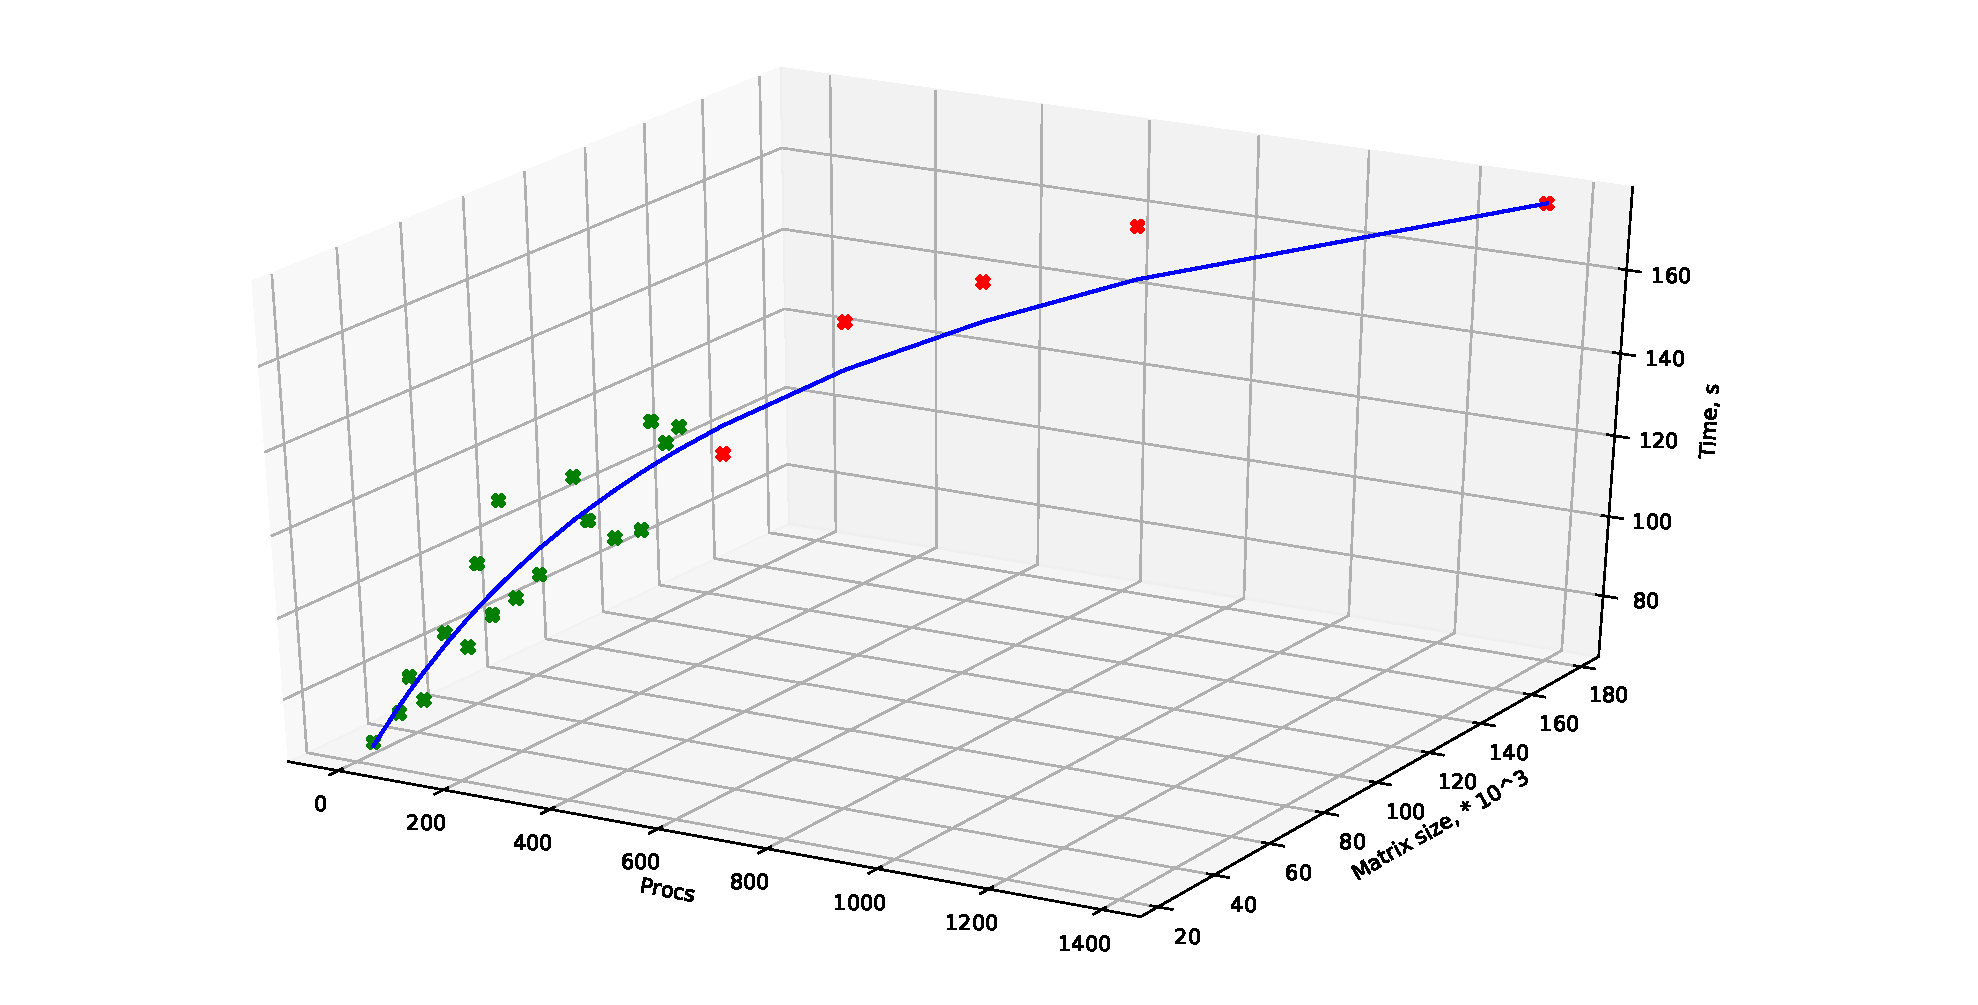
\includegraphics[width=0.9\textwidth]{hpl_k3}
		\caption{Аппроксимирующая функция для слабой масштабируемости HPL, конфигурации соответствуют константе \(C_3\)}
		\label{HPL_C_3_figure}
	\end{figure}

	Тестовые конфигурации запуска, используемые для вычислений параметров модели, и целевых конфигураций, необходимые для оценки погрешности предсказаний, приведены в таблицах \ref{test_HPL} и \ref{target_HPL} соответственно. Коэффициенты \(C_1, C_2, C_3\), связывающие количество работы приходящееся на один процесс и количество используемых процессов, из выражения \ref{weak_sc}, связаны отношением: \(4 \cdot C_1 = 2 \cdot C_2 = C_3 \), то есть с увеличением на единицу номера коэффициента количество работы на один процесс увеличивается в два раза.

	Относительные ошибки для всех целевых конфигураций слабой масштабируемости HPL представлены в таблице \ref{target_HPL}. Значения относительных ошибок предсказания времени по всем целевым конфигурациям варьируются от 0,02\% до 11,35\%, среднее значение - 4,12\%, медиана - 3,82\%, а производительности - от 0,07\% до 16,35\%, среднее значени - 5,23\%, медиана - 5,69\%. Если рассматривать более детально, как меняеются относительные ошибки с увеличением числа используемых процессов и размера задачи, усредняя значение ошибок по конфигурациям с одинаковым количеством использемых процессов, 225 - 5,09\%, 400 - 7,17\%, 576 - 3,74\%, 784 - 4,43\%, 1369 - 2,95\%, то можно однозначно сказать, что увеличение конфигурации, не приводит к росту значений относительных ошибок. 

	//////////////////говорить ли про рисунок и оставлять ли его вообще //////////////////////////////////////

	\section{HPCG}

	HPCG (High Performance Conjugate Gradients Benchmark) был разработан, чтобы стать альтернативым HPL метрикой оценки производительности суперкомпьютеров. Он сильно выделяется на фоне остальных приложений, так как и сложность последовательного алгоритма, и количество операций чтения/записи пропорциональны \(O(N)\). В тесте преобладают нерегулярный доступ к памяти и мелкострукрурные рекурсивные вычисления, которые свойственны многих научным вычислительным приложениям \cite{HPCG}. Основное вычислительное ядро HPCG занимается решением СЛАУ с разряженной положительно определённой симметричной матрицей с помощью метода сопряжённых градиентов.

	


	\section{Алгоритмы матричного умножения}
		\subsection{SUMMA}
		Первый из двух рассматриваемых алгоритмов матричного умножения - SUMMA(Scalable Universal Matrix Multiply)\cite{SUMMA}. Этот алгоритм используется такими библиотеками, как ScaLAPACK и PLAPACK.

		\subsection{DNS}

	\section{Graph500}
% \clearpage
	%\chapter{Заключение}
	В данной работе были получены следующие основные результаты:
	\begin{itemize}
		\item Разработан метод, предсказывающий слабую масштабируемость суперкомпьютерных приложений на основе экспериментальных данных.
		\item Выполнена проверка применимости метода на различных приложениях, с помощью запусков приложений HPL, HPCG, матричных алгоритмов умножения SUMMA и DNS, Graph500 на суперкомпьютере "<Ломоносов-2">.
	\end{itemize}

	На основании предложенного метода удалось построить предсказания слабой масштабируемости для всех рассматриваемых приложений так, что максимальная относительная ошибка среди всех приложений и конфигураций не превышает ???\%, а среднее значение относительной ошибки меняется от ???\% до ???\%. Таким образом, предложенный метод предсказания даёт относительные ошибки, сравнимые с ошибками предсказания у существующих подходов при сопоставимых размерах конфигураций предсказываемых запусков.

\clearpage
	\begin{thebibliography}{00}

	\bibitem{efficiency_prediction} 
	Rosas C., Giménez J., Labarta J. Scalability prediction for fundamental
	performance factors. Supercomputing Frontiers and Innovations, Vol 1, No 2,
	2014, p. 4-19

	\bibitem{simulation_FASE}
	FASE: A Framework for Scalable Performance Prediction of HPC Systems and Applications
	/ Grobelny E., Bueno D., Troxel I. et al. // SIMULATION. 2007. Vol. 83, No. 10. P. 721-745.

	\bibitem{representative_replay}
	Zhai J., Chen W., Zheng W., Li K. Performance Prediction for Large-Scale Parallel
	Applications Using Representative Replay // IEEE Transactions on Computers. 2016. Vol. 65,
	No. 7. P. 2184-2198.

	\bibitem{analytic_func}
	A. Calotoiu, T. Hoefler, M. Poke \& F. Wolf, "Using automated performance modeling
	to find scalability bugs in complex codes," SC '13: Proceedings of the International
	Conference on High Performance Computing, Networking, Storage and Analysis, Denver,
	CO, 2013, pp. 1-12

	\bibitem{log_main}
	A regression-based approach to scalability prediction / Barnes B. J., Rountree B., Lowenthal
	D. K. et al. // Proceedings of the ICS. 2008. P. 368-377.

	\bibitem{focused_regression}
	B. Barnes et al., "Using focused regression for accurate time-constrained scaling of scientific applications," 2010 IEEE International Symposium on Parallel and Distributed Processing (IPDPS), Atlanta, GA, 2010, pp. 1-12.

	\bibitem{UV_matrix}
	Q. Shao, L. Pan, S. Liu \& X. Liu, "A collaborative filtering based approach to performance prediction for parallel applications," 2017 IEEE 21st International Conference on Computer Supported Cooperative Work in Design (CSCWD), Wellington, 2017, pp. 331-336.

	\bibitem{ML_SMG2000}
	Ipek E., de Supinski B., Schulz M., McKee S. A. An approach to performance prediction for parallel applications // Euro-Par Parallel Processing. Lecture Notes in Computer Science. 2005. Vol. 3648. P. 196-205.

	\bibitem{ML_Grid}
	Nadeem, F., Alghazzawi, D., Mashat, A. et al. Modeling and predicting execution time of scientific workflows in the Grid using radial basis function neural network. Cluster Comput 20, 2805–2819 (2017).

	\bibitem{ML_PROC_KERN}
	Singh K. et al. (2010) Comparing Scalability Prediction Strategies on an SMP of CMPs. In: D’Ambra P., Guarracino M., Talia D. (eds) Euro-Par 2010 - Parallel Processing. Euro-Par 2010. Lecture Notes in Computer Science, vol 6271. Springer, Berlin, Heidelberg

	\bibitem{scaling_types}
	Антонов, А. С., Теплов, А. М. (2013). Исследование масштабируемости программ с использованием инструментов анализа параллельных приложений на примере модели атмосферы Nh3d. Вестник Южно-Уральского государственного университета. Серия: Вычислительная математика и информатика, 2 (1), 5-16.

	\bibitem{scalability_def}
	Alexander Antonov, Alexey Teplov. Generalized Approach to Scalability Analysis of Parallel Applications // Lecture Notes in Computer Science. Vol.10049, 2016. Pp. 291-304. DOI: 10.1007/978-3-319-49956-7\_23

  	\bibitem{top500}
  	The 54nd edition of the TOP500 list [Электронный ресурс]. – Электрон. дан. – URL: https://www.top500.org/lists/2019/11/. (дата обращения 16.03.2020).

	\bibitem{Kazmina_Antonov_article}
	К.П. Казьмина, А.С. Антонов. Разработка методов прогнозирования масштабируемости приложений на конфигурации суперкомпьютеров // Вестник компьютерных и информационных технологий. N 12, 2018. С. 45-56.(http://www.vkit.ru/index.php/current-issue-rus/770-045-056) DOI:10.14489/vkit.2018.12.pp.045-056

  	\bibitem{Kazminf_Valkon_Antonov_article}
    Pavel Valkov, Kristina Kazmina, and Alexander Antonov. Using Empirical Data for Scalability Analysis of Parallel Applications // Communications in Computer and Information Science. Vol. 1063. 2019. Pp. 58-73. DOI:10.1007/978-3-030-28163-2\_5

    \bibitem{Lom2_stat}
	Voevodin, V., Antonov, A., Nikitenko, D., Shvets, P., Sobolev, S., Sidorov, I., Stefanov, K., Voevodin, V., \& Zhumatiy, S. (2019). Supercomputer Lomonosov-2: Large Scale, Deep Monitoring and Fine Analytics for the User Community. Supercomputing Frontiers And Innovations, 6(2), 4-11. doi:http://dx.doi.org/10.14529/jsfi190201

	\bibitem{HPCG}
	Report, S., Dongarra, J., \& Heroux, M.A. (2013). Toward a New Metric for Ranking High Performance Computing Systems.
	
	\bibitem{SUMMA}
	Robert A. van de Geijn and Jerrell Watts. 1995. SUMMA: Scalable Universal Matrix Multiplication Algorithm. Technical Report. University of Texas at Austin, USA.




\end{thebibliography}
\clearpage

\end{document}